%%% Template for AUTHOR's DRAFT paper in FCAA, WITHOUT Journal's head  %%%%%%%%%%%%%%%%%%%%%%%%%%%%%%%%%
%%% by V. Kiryakova, updated Nov. 1, 2014
%%% uses "fcaa.cls", or "fcaa-var.cls" as modifications of "amsart.cls" for the FCAA format,
%%% and auxiliary file "fcaa_style.tex" fixing page margins, fontsize, defs for theorems, proofs etc.
%%% Put the files "fcaa.cls", "fcaa-var.cls" and "fcaa_style.tex" in same directory you prepare the paper

  %\documentclass[twoside,reqno,11pt]{fcaa}  %%% or in case of problems, use as below: %
  \documentclass[twoside,reqno,11pt]{fcaa-var} %

 \input fcaa_style

%%%%%%%%%%%%%%%%%%%%
 \usepackage{hyperref} % Editor will use to create hyperlinks %
 %%% but if the author has problems with the above style file,
 %%% then comment the line \usepackage{hyperref} or replace by this below:
 % \usepackage{upref}
%%%%%%%%%%%%%%%%%%%%

% to have 2-digits numbering for equation, use:
 \def\theequation{\arabic{section}.\arabic{equation}}

%%%%%%  First page footnote for Copyright and Springer logo
 \def\themycopyrightfootnote{\vspace*{3pt}
 \copyright \, Year\,  Diogenes  Co., Sofia
   \par  \noindent pp. xxx--xxx, DOI: ......................
   \hfill  \vspace*{-36pt}
   % \mbox{\includegraphics[scale=0.65]{DeGryuter.eps}}
  }
%%%%%%%%%%%%%%%%%%%%%%%%%%%%%%%%%%%%%%%%%%%%%%%%%%%%%%%%%%%%

  \setcounter{page}{1}
  \thispagestyle{empty}

 %%%%%%%%%%%%%%% begin make title %%%%%%%%%%%%%%%%%%%%%%%%%%%%%
 %%% TITLE: texts in [.] is abbreviated (1st line) title for running heads
 %%% Author(s): put in brackets [.] the short author's name

 \title[VISUALIZATION OF FRACTIONAL INTEGRALS]{VISUALIZATION OF THE RIEMANN-LIOUVILLE FRACTIONAL INTEGRAL \\ [3pt] IN ``FCAA'' JOURNAL}
 \author[\normalsize V. Kiryakova, S. Author]{\normalsize Virginia Kiryakova $^1$, Second Author $^2$}

 %%% obligatory give the full and abbreviated authors' names %%%
 %%%%%%%%%%%%%%%%%%%%%%%%%%%%%%%%%%%%%%%%%%%%%%%%%%%%%%%%%%%%%%%
                    % THE BEGINNING %
 \begin{document}

 \vbox to 2.5cm { \vfill }

%%% to make empty space of approx. 2.5cm %%%%%%
%%% will be replaced by Editor with the journal's and publoishers logos %%%%%%%%

 \bigskip \medskip

%%%% Abstract %%%%%%%%%%%%%%%%%%%%%%%%%
 \begin{abstract}

Text of the abstract. Text of the abstract. Text of the abstract.
Text of the abstract. Text of the abstract. Text of the abstract.
Text of the abstract. It should give a comprehensive idea about the
paper's subject and the author's results. The Abstract (and the first 2 pages of the paper) will be
available free at DeGryuter's website for the journal.

 \medskip

{\it MSC 2010\/}: Primary 26A33;
                  Secondary 33E12, 34A08, 34K37, 35R11, 60G22, ...

 \smallskip

{\it Key Words and Phrases}: fractional calculus, Mittag-Leffler
type functions, fractional ordinary and partial differential
equations, ...

 \end{abstract}

 \maketitle

%%%%%%% end make title %%%%%%%%%%%%%%%%%%%%%%%%%%%%%%%%%%
 \vspace*{-16pt}

%%%%%%%% begin papers' body %%%%%%%%%%%%%%%%%%%%%%%%%%%%%

%%%%%%%%%%%%%%%%%%%%%%%%%%% Section 1 %%%%%%%%%%%%%
%\section{Introduction}\label{Sec:1}

\section{First section of the paper}\label{sec:1}

\setcounter{section}{1}
\setcounter{equation}{0}\setcounter{theorem}{0}


Text ... (for details, see \cite{GasRah}, \cite{Rosbl}, \cite{Kir},
\cite{Moak}) ...

%%%% example of definition %%%%
 \begin{definition}\label{Def3}
Text of Definition~\ref{Def3}.
 \end{definition}

   \vspace*{-12pt} %%% example of subsection:
 \subsection{Preliminary results}\label{subsec:1.1}

%%%% example of theorem %%%%%%%%%%
 \begin{theorem}\label{Th1}
Text of Theorem~\ref{Th1} ....
 \end{theorem}

 \proof %%%%%%%%%%%%%
 Give here the proof of Theorem~\ref{Th1}. Example for
equation:
\begin{equation}\label{eq1}
ax^2+bx +c =0.
\end{equation}
 As seen by equation \eqref{eq1}, it is ...
 The proof follows from Ref. \cite{Moak}.
 \proofend %%%%%%%%%%

%%%% example of corollary %%%%
 \begin{corollary}\label{Cor2}
Text of Corollary~\ref{Cor2} ....
 \end{corollary}

 \proof
 Here comes the proof of Corollary~\ref{Cor2}.
 \proofend

%%%%%%%%%%%%%%%%%%%%%%%%%%%%%%%%%%%%%%%%%%%%%%%%%%
\section{Second section of the paper}\label{sec:2}

\setcounter{section}{2}
\setcounter{equation}{0}\setcounter{theorem}{0}


 Text ... As seen in Section~\ref{sec:1}, the equation
(\ref{eq1}), $ a\neq 0$, has the solutions
 \begin{equation}\label{eq2}
 x_{1,2}= {\frac {-b \pm \sqrt{b^2-4ac}}{2a}}\,.
 \end{equation}

 %%% example of example %%%%%
 \begin{example}\label{Ex1}
 Let us take in (\ref{eq2}) ... Then, by Theorem~\ref{Th1}, ...
 \end{example}

 \begin{example}\label{Ex2}
 Under same conditions as in Example~\ref{Ex1}, we consider ...
 \end{example}


The figures should be input in the LaTeX file as eps-files, as below:

%%%%%%%%% example for figure %%%%%%%%%%%%%%%%%%%
  \begin{center}
  \includegraphics[scale=0.4]{figure.eps}
 % \hspace*{2cm}
 % \includegraphics[scale=0.7]{figure2.eps}

 \bigskip

  Fig. 2.1: Control loop
  \end{center}
%%%%%%%%%%%%%%%%%%%%%%%%%%%%%%%%%%%%%%%%%%%%%%%

 Often figures include texts or Latin, Greek etc. letters.
 We kindly ask the authors to take care that no texts fonts need to be embedded, by saving first the text as curves.
 Just in case, along with the obligatory eps-files, please send us also some alternative figures' files in  pdf-, jpg-, etc. format.

\section{Riemann-Stieltjes integral}
Let $f$ and $g$ denote real-valued functions defined on a closed interval $[a',b']$ of the real line. We shall suppose that both $f$ and $g$ are bounded on $[a',b']$. These assertions are assumed to be true throughout the paper and will not be repeated again.

\begin{definition}
Define a partition $\mathcal{P}$ of $[a',b']$ to be a set of points $x_0, x_1,\cdots,x_n$, 
where $a' = x_0 \leq x_1 \leq \cdots \leq x_n = b'$. For each partition 
$\mathcal{P}$ of $[a',b']$ write $\Delta g_k = g(x_k)-g(x_{k-1})$. Let 
$M_k = \sup\{f(x),x_{k-1}\leq x \leq x_{k}\}$, $m_k = \inf\{f(x),x_{k-1}\leq x \leq x_{k}\}$, and set 
\begin{equation}
\label{ref:S_up}
\mathcal{S}_U(\mathcal{P},f,g) = \sum_{k=1}^n M_k \Delta g_k, 
\end{equation}
and
\begin{equation}
\label{ref:S_low}
\mathcal{S}_L(\mathcal{P},f,g) = \sum_{k=1}^n m_k \Delta g_k. 
\end{equation}
The sums in Eq.~\eqref{ref:S_up} and Eq.~\eqref{ref:S_low} are respectively called the the upper and lower Riemann-Stieltjes sums.
If there is a unique number $I$ that satisfies the inequality $\mathcal{S}_L(\mathcal{P},f,g)\leq I \leq \mathcal{S}_U(\mathcal{P},f,g)$ for all 
partitions $P$ of $[a',b']$, then $f$ is Riemann integrable with respect to $g$ on $[a',b']$. Moreover, $I$ is called the Riemann-Stieltjes integral of $f$ from $a'$ to $b'$ and is denoted by
\begin{equation}
\int_{a'}^{b'} f(x) dg(x). 
\end{equation}
\end{definition}

\begin{theorem}
If the derivative $g'$ exists and is continuous on $[a',b']$ and if $f$ is integrable with respect to $g$ on $[a',b']$, then the following 
Riemann and Riemann-Stieltjes integrals are equivalent
\begin{equation}
\int_{a'}^{b'} f(x) dg(x) = \int_{a'}^{b'} f(x)g'(x)dx.
\end{equation}
\end{theorem}
 
 
\section{Cavalieri Integral}
\label{sec:cav_integral}

Ackerman et al. used the notion of non-rectangular integration strips to define the so called Cavalieri integral. The area of a non-rectangular 
integration strip is calculated using Cavalieri's principle. Cavalieri's principle is stated below without proof:
\begin{theorem}
Suppose two regions in a plane are included between two parallel lines in that plane. If every line parallel to these
two lines intersects both regions in line segments of equal length, then the two regions have equal areas. NEED CITATION
\end{theorem}
The definition of the Cavalieri integral is presented in Definition~\ref{def:cav_integral}.
It is, however, our experience that Definition~\ref{def:cav_integral} is hard to assimilate if it is encounterd by a reader for the first time. We, therefore, encourage 
readers who are not familiar with the Cavalieri integral to rather first read Section~\ref{??} instead. The reader who is not familiar with the Cavalieri integral should only refer back to the definitions 
presented in this section when things in Section~\ref{??} become unclear. Moreover, the definitions presented below were taken from [?]. Furthermore, none of the theorems in this section are proved, the proofs can be found in [].

\begin{definition}\label{def:trans}
A continuous real--valued function $a(y)$ is called a translational function with respect to a continuous real--valued function $f(x)$ on the interval $[a,b]$ if 
$\{x\in\mathbb{R}|a\circ f(x) + z = x\}$ is a singleton, for every $z\in[0,b-a]$ and $a(0) = a$.
\end{definition}

Let $a(y)$ be a translational function with respect to a real--valued function $f(x)$ on the interval $[a,b]$. Moreover, $b(y) = a(y) + (b-a)$. Furthermore, the functions $a(y)$ and $b(y)$ intersect $f(x)$ at $a'$ and $b'$ respectively.
These assertions are assumed to be true throughout the paper and will not be repeated again.

\begin{definition}\label{def:h}
The mapping $h : [a, b] \rightarrow [a',b']$, which maps $x_i^1 \in [a, b]$ to $x_i^2 \in [a',b']$, is defined as
$h(x_i^1) =$ $\{x_i^2 \in [a' ,b'] | a\circ f(x_i^2) + [x_i^1 - a] = x_i^2$ , $a = a(0)\}$
\end{definition}

\begin{definition}\label{def:g}
The mapping $g:[a', b'] \rightarrow [a, b]$, which maps $x_i^2 \in [a' , b']$ to $x_i^1\in [a, b]$,
is defined as $g(x_i^2) = x_i^2 - a \circ f (x_i^2) + a$.
\end{definition}

\begin{theorem}
The mapping $h(x)$ is a strictly monotone continuous function. The function $h(x)$ is, therefore, invertable.
\end{theorem}

\begin{theorem}
\label{t:inv}
The function $g(x)$ is equal to $h^{-1}(x)$.
\end{theorem}

\noindent
The functions $h(x)$ and $g(x)$ are known as the transformation function and the inverse transformation function, respectively. 

\begin{definition}\label{def:cav_integral}
Define a partition $\mathcal{P}_1$ of $[a,b]$ to be a set of points $x_0^1, x_1^1,\cdots,x_n^1$, 
where $a = x_0^1 \leq x_1^1 \leq \cdots \leq x_n^1 = b$. For each partition 
$\mathcal{P}_1$ of $[a,b]$ write $\Delta x_k^1 = x_k^1-x_{k-1}^1$. 
%Since both boundaries of any integration strip are necessarily
%translations of the translational function $a(y)$, we can apply the transformation
%function $h$ to the partition $\mathcal{P}_1$. 
If the transformation function $h$ is strictly increasing,
the application of $h$ to the partition $\mathcal{P}_1$ induces a new partition $\mathcal{P}_2 = \{x_0^2, x_1^2,\cdots, x_n^2\}$.
Otherwise, if $h$ is strictly decreasing, the application of $h$ induces a reversed partition $\mathcal{P}_2 = \{x_n^2, \cdots, x_1^2,x_0^2\}$. It
can be assumed that $h$ is strictly increasing, without any loss of generality.  Let 
$M_k = \sup \{f (x), h(x_{i-1}^1) = x_{i-1}^2 \leq x \leq x_i^2 = h(x_i^1)\}$, $m_k = \inf \{f (x), h(x_{i-1}^1) = x_{i-1}^2 \leq x \leq x_i^2 = h(x_i^1)\}$, and set 
\begin{equation}
\label{eq:c_up}
\mathcal{C}_U(\mathcal{P}_1,f,h) = \sum_{k=1}^n M_k \Delta x_k^1, 
\end{equation}
and
\begin{equation}
\label{eq:c_low}
\mathcal{C}_L(\mathcal{P}_1,f,h) = \sum_{k=1}^n m_k \Delta x_k^1. 
\end{equation}
The sums in Eq.~\eqref{eq:c_up} and Eq.~\eqref{eq:c_low} are respectively called the the upper and lower Cavalieri sums.
If there is a unique number $I$ that satisfies the inequality $\mathcal{C}_L(\mathcal{P}_1,f,h)\leq I \leq \mathcal{C}_U(\mathcal{P}_1,f,h)$ for all 
partitions $\mathcal{P}_1$ of $[a,b]$, then $I$ is called the Cavalieri integral of $f$ from $a(y)$ to $b(y)$ and is denoted by
\begin{equation}
\int_{a(y)}^{b(y)} f(x) dx.
\end{equation}
\end{definition}

Note that the superscripts of the $x$-coordinates in the above definitions indicate to which partition, either $\mathcal{P}_1$ or $\mathcal{P}_2$, the $x$-coordinate in question belongs.

\begin{theorem}
\label{t:conv}
The following Cavalieri, Riemann, and Riemann--Stieltjes integrals are equivalent:
\begin{equation}
\int_{a(y)}^{b(y)} f(x)\,dx = \int_a^b f\circ h(x)\,dx = \int_{a'}^{b'} f(x)\,dg(x),
\end{equation}
with $g(x) = x-a\circ f(x) + a$ and $h(x) = g^{-1}(x)$.
\end{theorem}

Theorem~\ref{t:conv} tells us how to convert a Cavalieri integral into an equivalent Riemann or Riemann-Stieltjes integral. It, however, tells us nothing about the reverse 
procedure, if we are given a Riemann-Stieltjes integral how do we convert it into a Cavalieri integral. The theorem below stipulates the conditions that are required to perform the latter conversion.

\begin{definition}
The Riemann-Stieltjes integral $\int_{a'}^{b'} f(x)\,dg(x)$ and the Cavalieri integral $\int_{a(y)}^{b(y)}f(x)\,dx$ are said to be geometrically equivalent if the same result is obtained when they are evaluated, $g(a')=a(0)=a$ and $g(b')=b(0)=b$. 
\end{definition}

Please note that the integrals in the above definition refer to two randomly 
chosen integrals and not integrals that were obtained via Theorem~\ref{t:conv}. Integrals
obtained using Theorem~\ref{t:conv} are geometrically equivalent by definition.
We used the same notation in the above definitiion as that used in Theorem~\ref{t:conv} as we believe that this improves the readability and the interpretability of later definitions and theorems.

\begin{theorem}
\label{t:reverse}
Let $\widetilde{g}(x)$ be a known continuous, differentiable and invertable real-valued function on $[a',b']\subset\mathbb{R}$. Let $f(x)$ be a continious real-valued function.  If $a(y)=f^{-1}(y) - \widetilde{g}\circ f^{-1}(y) + \widetilde{g}(a')$ and $a(0)$ exists then there exists a unique $C\in\mathbb{R}$ such that 
\begin{equation}
\int_{a'}^{b'} f(x)\,dg(x)~\textrm{and}~\int_{a(y)}^{b(y)} f(x)\,dx, 
\end{equation}
where $g(x) = \widetilde{g}(x) + C$, are geometrically equivalent.
\end{theorem}

To clarify the above theorem, consider the Riemann-Stieltjes integral $\int_{a'}^{b'} f(x)\,d\,\widetilde{g}(x)$. The Cavalieri-Stieltjes integral pair associated with this Stieltjes integral can only be determined if $C$ is known to us. Luckily, this can be easily obtained using the the following steps (taken from \cite{??}):
\begin{itemize}
 \item Compute $a(y)$ using: 
\begin{equation}
a(y) = f^{-1}(y)-\widetilde{g}\circ f^{-1}(y) + \widetilde{g}(a'). 
\end{equation}
 \item Compute $a = a(0)$.
 \item Compute $C = a - \widetilde{g}(a')$.
 \item Compute $g(x) = \widetilde{g}(x) + C$.
 \item Compute $b = g(b')$ and $b(y) = a(y) + (b-a)$.
\end{itemize}
Note that $\int_{a'}^{b'} f(x)\,d\,\widetilde{g}(x)=\int_{a'}^{b'} f(x)\,dg(x)$ due to Theorem xx. Moreover, the integrals $\int_{a'}^{b'} f(x)\,d\,g(x)$ and $\int_{a(y)}^{b(y)}f(x)~dx$ are geometrically equivalent. Note, however, that
$\int_{a'}^{b'} f(x)\,d\,\widetilde{g}(x)$ and $\int_{a(y)}^{b(y)}f(x)~dx$ are not geometrically equivalent.

The theorems and definitions presented in this section impose much greater restrictions on $g(x)$ and $f(x)$ than that mentioned in the begining of Section. The functions 
$g(x)$, $\widetilde{g}(x)$ and $f(x)$ now also need to be differentiable and invertable. Moreover, the function $a(y)$ also needs to be differentiable and $a(0)$ needs to exist.
These assertions are deemed to be true for the remainder of the paper and as such are not repeated again. As will become clear later on, these restrictions limit the number of fractional integrals for which the geometric framework we propose in this paper can produce meaningful results. This, however, does not diminish the importance of the proposed framework, since, for the integrals for which it does produce meaningful results, it will lead to new and novel insights.


%To clarify the above theorem, the Riemann-Stieltjes integral $\int_{a'}^{b'} f(x)\,d\,\widetilde{g}(x)$ can be converted into an equivalent Cavalieri integral $\int_{a(y)}^{b(y)}f(x)~dx$ (we obtain the same value when we evaluate the aforementioned integrals). The Cavalieri 
%integral so obtained does however not have the same geometric meaning as $\int_{a'}^{b'} f(x)\,d\,\widetilde{g}(x)$. Fortunately, the Riemann-Stieltjes integral $\int_{a'}^{b'} f(x) \,d\,\widetilde{g}(x)$ 
%can be converted into an equivalent Riemann-Stieltjes integral $\int_{a'}^{b'} f(x)\,dg(x)$. Note that $\int_{a'}^{b'} f(x)\,d\,\widetilde{g}(x) = \int_{a'}^{b'} f(x)\,dg(x)$, by Theorem~\ref{??}. In contrast to the original Riemann-Stieltjes integral, the Riemann-Stieltjes integral so obtained has the exact same geometric meaning as $\int_{a(y)}^{b(y)} f(x)\,dx$.


\section{Cavalieri Integral: Clarifying Example}
\label{sec:cav_integral_example}
The example which we present below was taken from \cite{?}. Let the region $R$ be bounded by the $x$-axis and the lines $f(x)=x$, $a(y)=1-y$ and $b(y)=4-y$. This region is depicted in Fig.~\ref{fig:caval2}.\\
%\begin{figure}[htb]
%\centering
%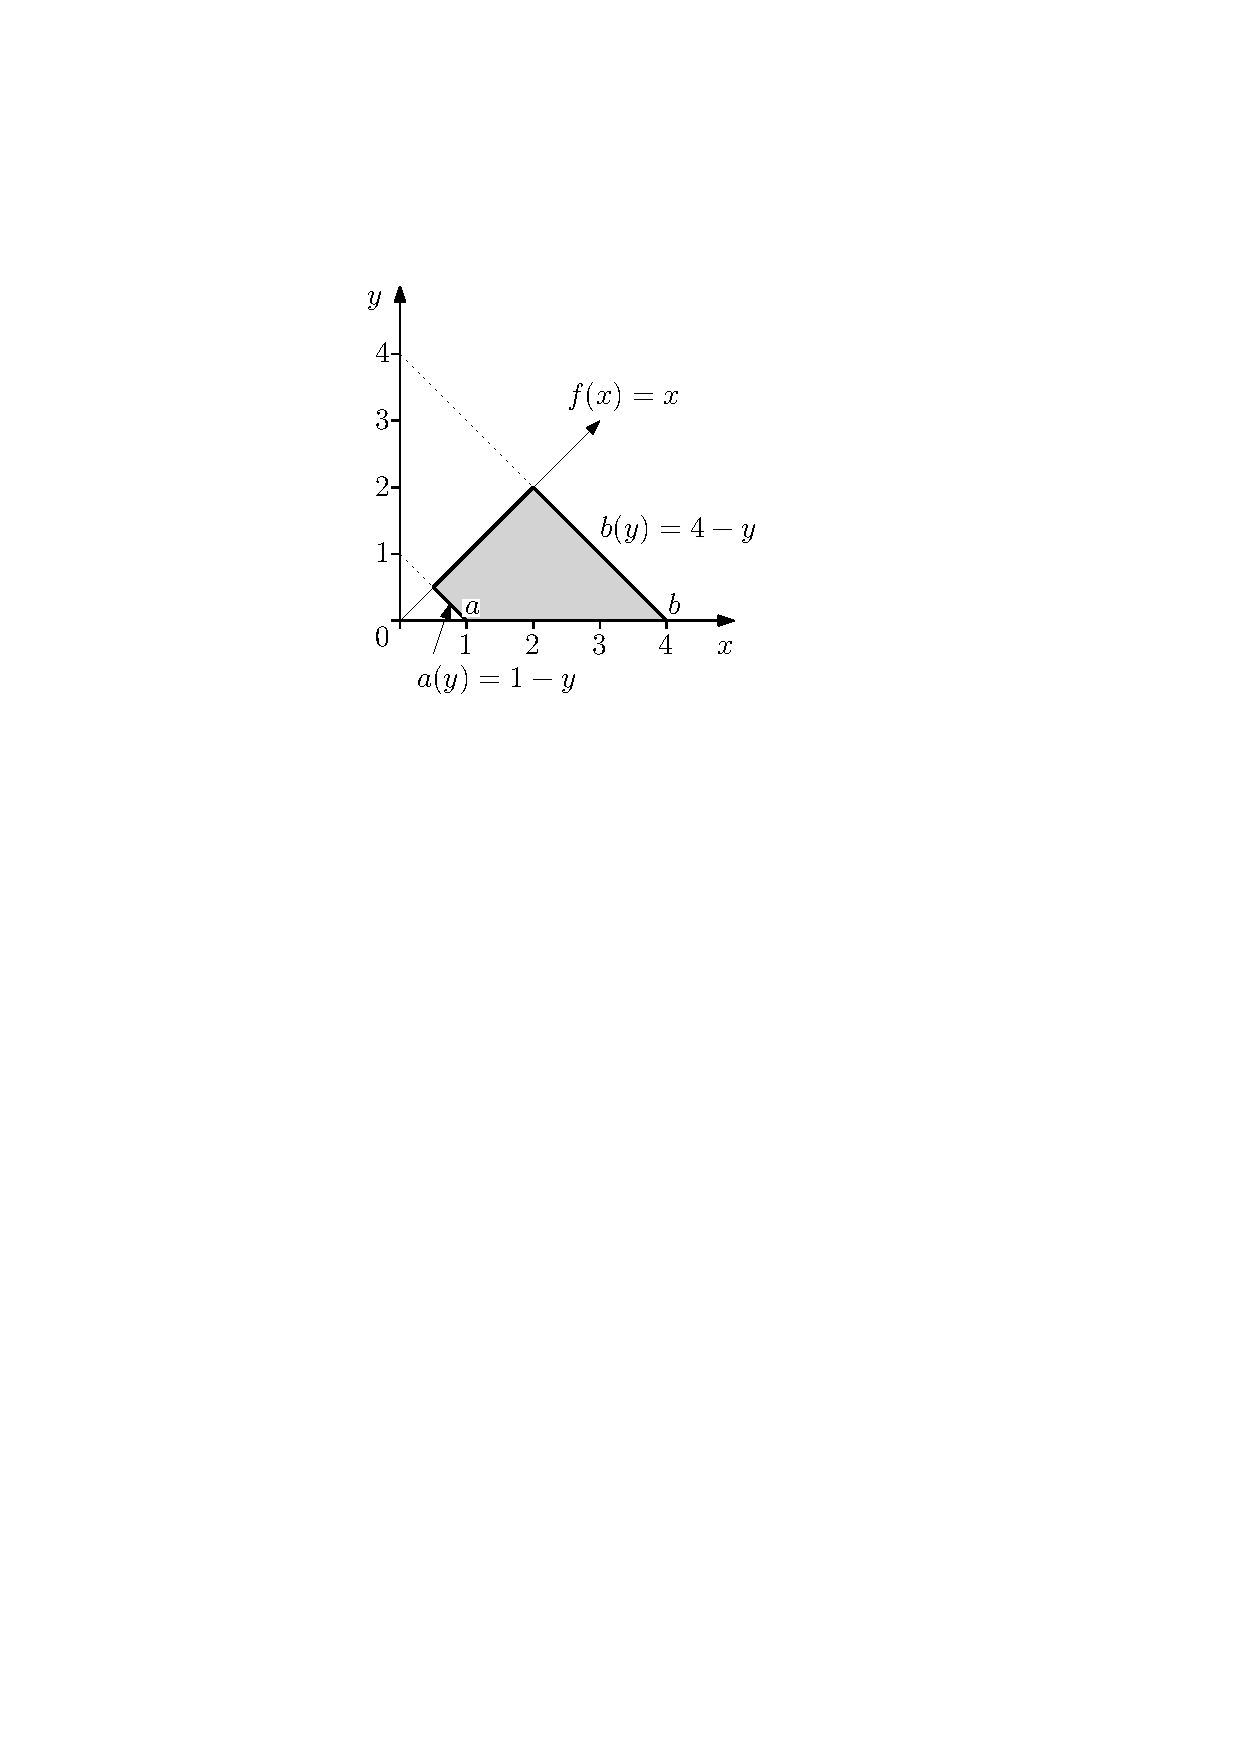
\includegraphics[width=0.3\textwidth]{fig12}
%\caption{Region bounded by the $x$-axis and the lines $f(x)=x$, $a(y)=1-y$, and $b(y)=4-y$. Reproduced from Quaestiones Mathematicae (2012) 35: 265-296 with permission \copyright~ NISC (Pty) Ltd.}
%\label{fig:ex1}
%\end{figure}
%\begin{figure}[htb]
%\centering
%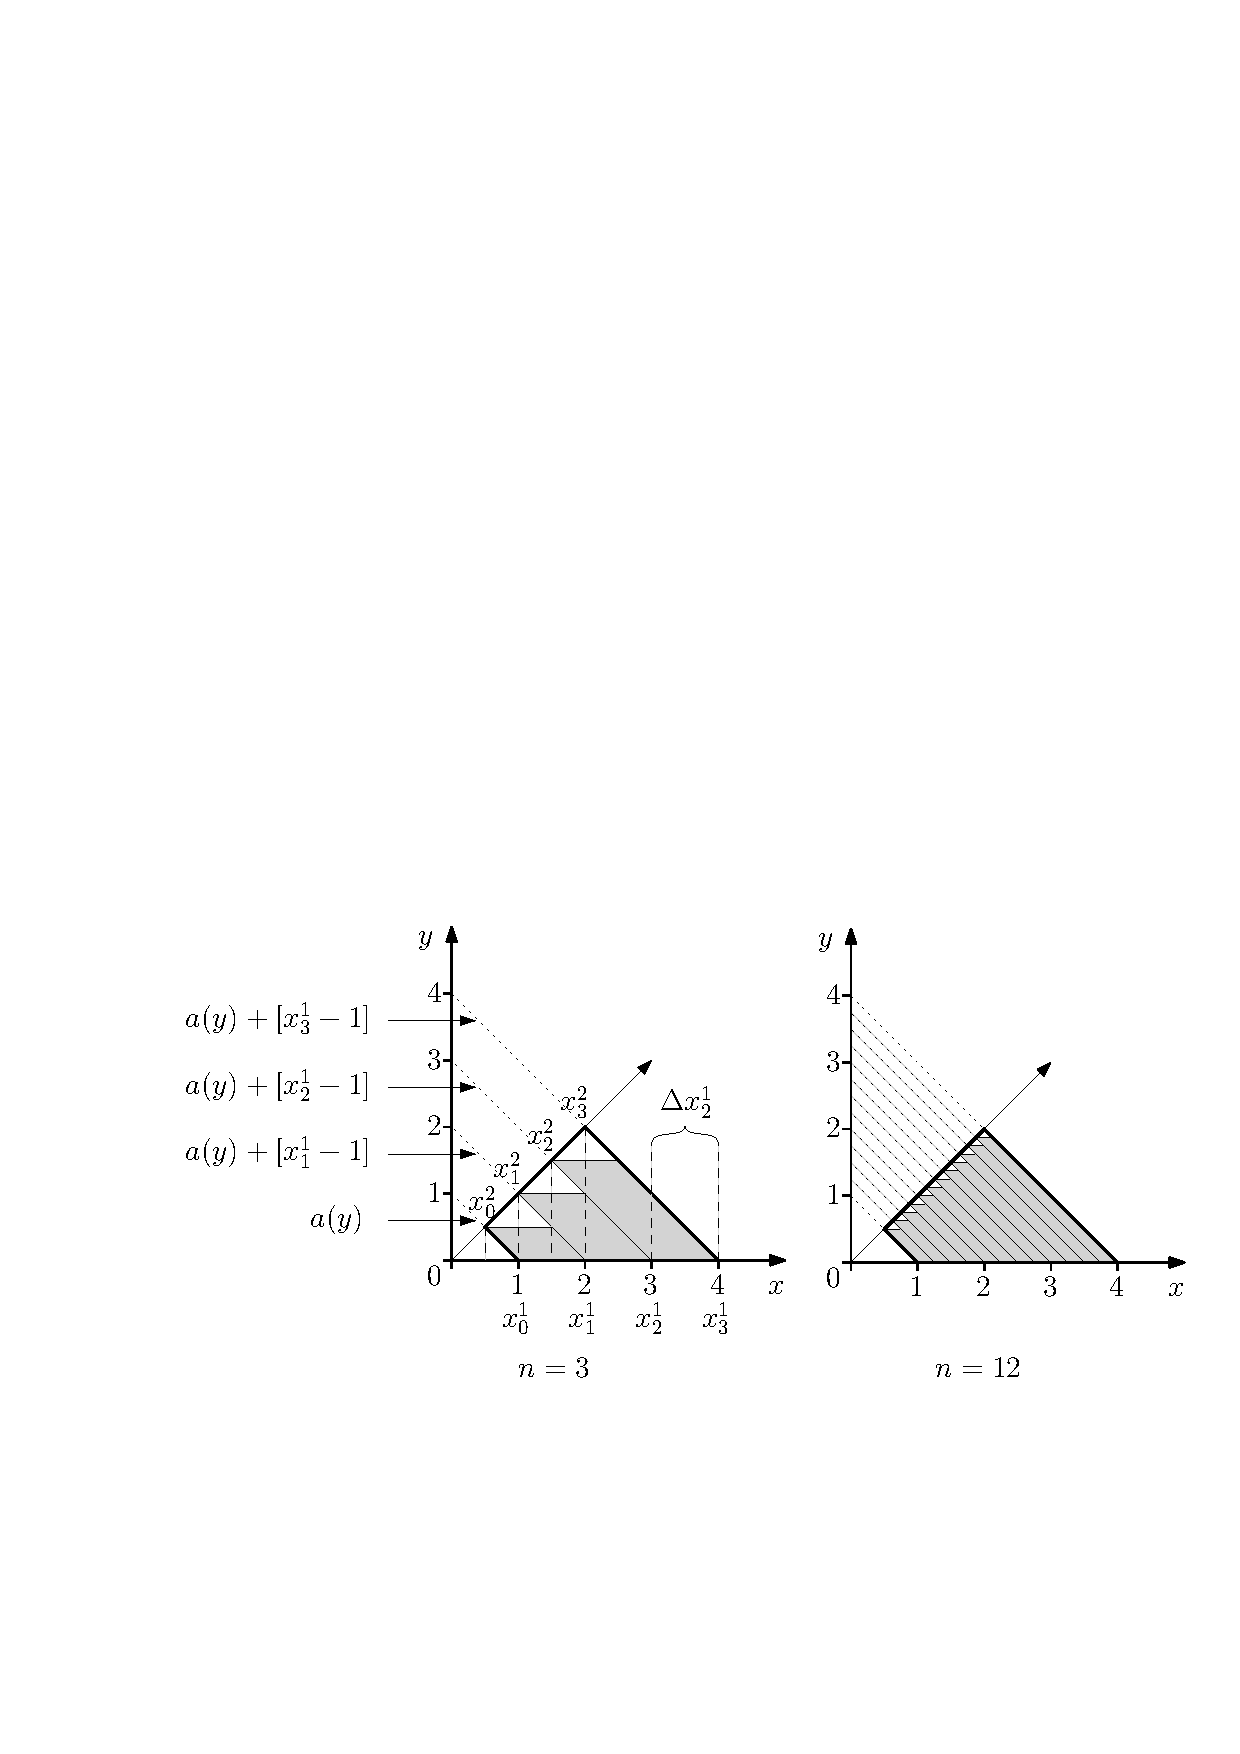
\includegraphics[width=0.75\textwidth]{fig13.pdf}
%\caption{Region bounded by the $x$-axis and the lines $f(x)=x$, $a(y)=1-y$, and $b(y)=4-y$. In the case of $R$: $a=1$, $b=4$, $a'=\frac{1}{2}$ and $b'=2$. The figure also depicts the partition points $x_i^2$ as used in the Cavalieri sum (see Equation~\eqref{eq:cav_sum}). Reproduced from Quaestiones Mathematicae (2012) 35: 265-296 with permission \copyright~ NISC (Pty) Ltd.}
%\label{fig:caval2}
%\end{figure}

%\noindent
%The area of $R$ can be determined as follows if we employ the classical notion of integration:
%\begin{equation}
%\int_0^2x\, dx+\int_2^44-x\, dx- \int_0^{\frac{1}{2}}x\, dx-\int_{\frac{1}{2}}^11-x\, dx = 3.75. 
%\end{equation}

We can approximate the area of $R$ by using rectangular integration strips. It, however, seems much more straightforward to approximate the area of $R$ via non-overlapping non-rectangular integration strips that toghether inscribe $R$. This alternative approach 
will only succeed it the sides of the aforementioned integration strips are all tranlsations of the function $a(y)$. 

Let us express this idea more formally. Let $(x_i^1)_{i=0}^{n}$ denote a partition on the $x$-axis, such that $a = x_0^1 < x_1^1 < \cdots < x_n^1 = b$, and $\Delta x_i^1 = x_{i+1}^1 - x_i^1$.
We are now able to construct the following lower Cavalieri sum (Equation~\ref{eq:c_low}):
\begin{equation}
\label{eq:cav_sum}
\sum_{i=0}^{n-1} f(x_i^2)\Delta x_i^1.
\end{equation}
The partition points $(x_i^2)_{i=0}^{n}$ are depicted in Fig.~\ref{fig:caval2}. Cavalieri's principle tells us that the area of integration strip $i$ is equal to $f(x_i^2)\Delta x_i^1$. Equation.~\eqref{eq:cav_sum}, therefore, approximates the area of $R$. In the limit Eq.~\eqref{eq:cav_sum} approaches 
the Cavalieri integral (Definition~\ref{def:cav_integral}):
\begin{equation}
\label{eq:caval1}
\int_{a(y)}^{b(y)}f(x)\, dx = \lim_{n\to \infty}\sum_{i=0}^{n-1} f(x_i^2)\Delta x_i^1.
\end{equation}
It is, however, quite hard to evaluate the above integral directly. Fortunately, it is easy to convert a Cavalieri integral into an equivalent Riemann or Riemann-Stieltjes 
integral by using the functions $h$ and $g$ (Theorem~\ref{t:conv}). Expressed mathematically:
\begin{equation}
\label{eq:main_cav}
\int_{a(y)}^{b(y)}f(x)\,dx =\int_a^b f \circ h (x)\, dx = \int_{a'}^{b'} f(x) dg(x),
\end{equation}
We can calculate $g$ as follows (Definition~\ref{def:g}):
\begin{equation}
g(x) = x - a\circ f(x) + a.
\end{equation}
Moreover, $h=g^{-1}$ (Theorem~\ref{t:inv}). We can now evaluate the Cavalieri using one of two ways:
\begin{equation}
\int_{a(y)}^{b(y)}f(x)\, dx = \int_a^b f \circ h (x)\, dx = \dfrac{1}{2}\int_1^4x\, dx = 3.75,  
\end{equation}
or
\begin{equation}
\int_{a(y)}^{b(y)}f(x)\, dx = \int_{a'}^{b'} f \, dg(x) = \int_{\frac{1}{2}}^2x\, d2x = 3.75.  
\end{equation}
Note, that in the above two equations: $h(x) = \frac{1}{2}x$ and $g(x) = 2x$. 

We can easily verify that the above is correct by using a more traditional route:
\begin{equation}
\int_0^2x\, dx+\int_2^44-x\, dx- \int_0^{\frac{1}{2}}x\, dx-\int_{\frac{1}{2}}^11-x\, dx = 3.75. 
\end{equation}

Conversely, consider the following Riemann-Stieltjes integral:
\begin{equation}
\int_{a'}^{b'} \,d\,\widetilde{g}(x) = \int_{\frac{1}{2}}^2 x\,d2x.
\end{equation}
We can convert this Riemann-Stieltjes integral into a Cavalieri integral via the following conversion steps (see Theorem~\ref{??} and the last paragraph of Section~\ref{??}):
\begin{itemize}
 \item $a(y) = f^{-1}(y) - \widetilde{g}\circ f^{-1}(y)+ \widetilde{g}(a') = 1-y$.
 \item $a(0) = 1$.
 \item $C = a - \widetilde{g}(a') = 0$.
 \item $g(x) = \widetilde{g}(x) + C = 2x$.
 \item $b = g(b') = 4$ and $b(y) = a(y) + (b-a) = 4-y$.
\end{itemize}
The integrals $\int_{\frac{1}{2}}^{2} x\,d2x$  and $\int_{1-y}^{4-y} x\,dx$ have the exact same geometric meaning, since $C=0$. 

\section{Left-sided Riemann-Liouville Fractional Integral}
In this section we review the definition of the left-sided Riemann-Liouville fractional integral of order $\alpha$ (based at $a'$) \cite{laurent1884}. Let
\begin{equation}
_{a'}I_t\, f(t) := \int_{a'}^t f(\tau)~d\tau.
\end{equation}
Please note that in this paper from this point going forward our variable of integration will be $\tau$ instead of $x$. It is of our opinion that this notational change improves the readability of the paper (if $\tau$ is our variable of integration then it makes sense to choose $t$ to denote our upper integration limit in Eq.~\ref{??}). 
If we apply the above operator in a repetitive manner to $f$ we obtain the $n$th antiderivative of $f$ based at $a'$:
\begin{equation}
\label{eq:n_anti}
_{a'}I_t^n\,f(t) = \int_{a'}^t\int_{a'}^{\tau_1}\cdots \int_{a'}^{\tau_{n-1}}f(\tau_n)~d\tau_n\cdots d\tau_2 d\tau_1.
\end{equation}
Applying Cauchy's repetitive integration formula to Eq.~\eqref{eq:n_anti} results in:
\begin{equation}
\label{eq:cauchy}
_{a'}I_t^n\,f(t) = \frac{1}{(n-1)!}\int_{a'}^t (t-\tau)^{n-1}f(\tau)~d\tau.
\end{equation}
As an example if $f(t)=t$, $n=2$ and $a'=0$ then Eq.~\eqref{eq:cauchy} reduces to:
\begin{equation}
_{0}I_t^2\,f(t) = \int_0^t (t-\tau)\tau~d\tau = \frac{\tau^2 t}{2} - \frac{\tau^3}{3} \Bigg |_0^t = \frac{t^3}{3!}.
\end{equation}
The definition in Eq.~\eqref{eq:cauchy} can now be extended to an arbitrary fractional order by replacing $(n-1)!$ with the Gamma function (see Fig.~\ref{fig:gamma}):
\begin{equation}
\label{eq:frac_integral}
_{a'}I_t^{\alpha}f(t) = \frac{1}{\Gamma(\alpha)}\int_{a'}^t (t-\tau)^{\alpha-1}f(\tau)~d\tau.
\end{equation}
Eq.~\eqref{eq:frac_integral} is known as the left-sided Riemann-Liouville fractional integral of order $\alpha$. As an example if $f(t)=t$, $\alpha=\frac{1}{2}$ and $a'=0$ then 
Eq.~\eqref{eq:frac_integral} reduces to:
\begin{equation}
_0 I_t^{\frac{1}{2}}\,f(t) = \frac{1}{\Gamma(\frac{1}{2})} \int_0^t \frac{\tau}{\sqrt{t-\tau}} d\tau = \frac{1}{\sqrt{\pi}}\left [ -\frac{2}{3}\sqrt{t-\tau}(2t+\tau)\right] \Bigg |_0^t=\frac{4}{3\sqrt{\pi}}t^{\frac{3}{2}}. 
\end{equation}

\begin{figure}[htb]
\centering
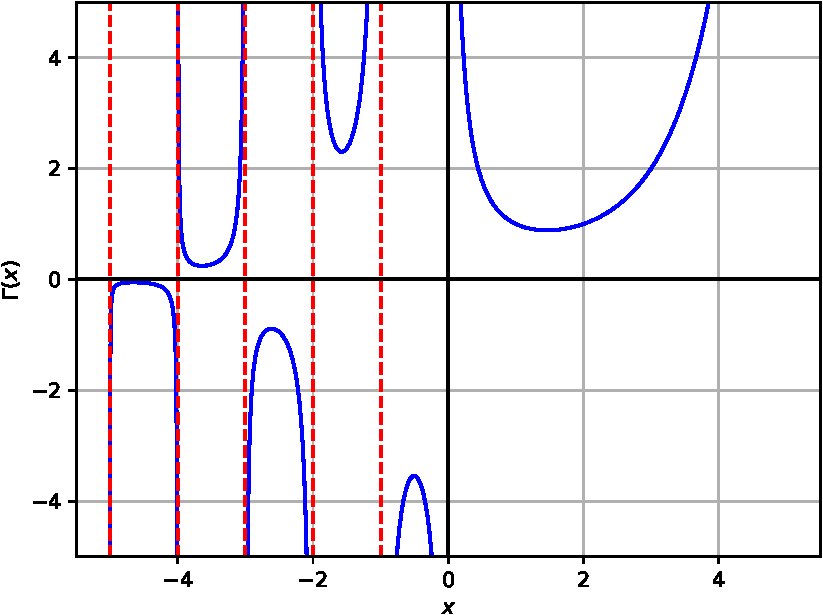
\includegraphics[width=0.75\textwidth]{gamma.pdf}
\caption{A plot of $\Gamma(x) = \int_0^{\infty} t^{x-1} e^{-t}\,dt$ for $x\in(-5,5)$. $\Gamma(x)$ is not defined for the negative integers. Moreover, it is a natural extension of the factorial function to the real numbers \cite{euler1738}.}
\label{fig:gamma}
\end{figure}

\section{Geometric Interpretation of the Left-sided Riemann-Liouville Fractional Integral}

\subsection{Converting into a Riemann-Stieltjes integral}
Podlubny showed that the Left-sided Riemann-Liouville fractional integral can be rewritten as a Riemann-Stieltjes integral \cite{podlubny02}:
\begin{theorem}
Let $C\in\mathbb{R}$. The following integrals are equivalent
\begin{equation}
_{a'}I_t^{\alpha}\,f(t) = \frac{1}{\Gamma(\alpha)}\int_{a'}^{t}(t-\tau)^{\alpha-1}f(\tau)~d\tau = \int_{a'}^{t} f(\tau)~dg_t^{\alpha}(\tau), 
\end{equation}
with 
\begin{equation}
\label{eq:g_rl}
g_t^{\alpha}(\tau) = \frac{\left \{t^{\alpha} - (t-\tau)^{\alpha} \right \}}{\Gamma(\alpha+1)} + C. 
\end{equation}
\end{theorem}

\begin{proof}
Note that 
\begin{equation}
\label{eq:diff}
\frac{dg_t^{\alpha}(\tau)}{d\tau} = \frac{\alpha(t-\tau)^{\alpha-1}}{\Gamma(\alpha+1)} =\frac{(t-\tau)^{\alpha-1}}{\Gamma(\alpha)}. 
\end{equation}
Furthermore,
\begin{equation}
\label{eq:inter_step}
\int_{a'}^{t} f(\tau)\,dg_t^{\alpha}(\tau) = \int_{a'}^{t} f(\tau) \frac{dg_t^{\alpha}(\tau)}{d\tau}\,d\tau. 
\end{equation}
The desired result is obtained by substituting Equation~\eqref{eq:diff} into Equation~\eqref{eq:inter_step}.  
\end{proof}

\begin{theorem}
The function $g_t^{\alpha}(\tau)$ is invertable. Its inverse is:
\begin{equation}
h_t^{\alpha}(\tau) = t - \sqrt[\alpha]{t^{\alpha} - \Gamma(\alpha+1)(\tau-C)}.
\end{equation}
\end{theorem}
\begin{proof}
The function $g_t^{\alpha}$ is invertable, since $\frac{d g_t^{\alpha}}{d\tau}=\frac{(t-\tau)^{\alpha-1}}{\Gamma(\alpha)} > 0$ for $\tau\in(-\infty,t]$. The inverse now follows trivially.  
\end{proof}

\noindent
Let $\mathsf{A} = \{0,0.2,0.4,0.6,0.8,1\}$. The analytic expressions of $g_{10}^{\alpha}(\tau)$ and $h_{10}^{\alpha}(\tau)$ are presented in Table~\ref{tab:gandh} for $\alpha\in\mathsf{A}$. 
The expressions in Table~\ref{tab:gandh} are depicted in Fig~\ref{fig:gandh}.

\begin{table}[h!]
 \centering
 \caption{The analytic expressions of $g_{10}^{\alpha}(\tau)$ and $h_{10}^{\alpha}(\tau)$ for $\alpha\in\mathsf{A}$. The expressions in this table are depicted in Fig~\ref{fig:gandh}.}
 \label{tab:gandh}
 \begin{tabular}{|c || c | c|} 
 \hline
 $\alpha$ & $g_{10}^{\alpha}(\tau)$ & $h_{10}^{\alpha}(\tau)$ \\ [0.5ex] 
 \hline\hline
 $0$ & 0 & $y=0$ \\ 
 $0.2$ & $[\Gamma\left (\frac{6}{5} \right )]^{-1}\left(\sqrt[5]{10}-\sqrt[5]{10-\tau}\right)$ & $10 - \left ( \sqrt[5]{10} -  \Gamma\left (\frac{6}{5} \right ) \tau \right )^5$  \\
 $0.4$ & $[\Gamma\left (\frac{7}{5} \right )]^{-1}\left(\sqrt[5]{10^2}-\sqrt[5]{(10-\tau)^2}\right)$ & $10 - \sqrt{\left ( \sqrt[5]{10^2} -  \Gamma\left (\frac{7}{5} \right ) \tau \right )^5}$ \\
 $0.6$ & $[\Gamma\left (\frac{8}{5} \right )]^{-1}\left(\sqrt[5]{10^3}-\sqrt[5]{(10-\tau)^3}\right)$ & $10 - \sqrt[3]{\left ( \sqrt[5]{10^3} -  \Gamma\left (\frac{8}{5} \right ) \tau \right )^5}$ \\
 $0.8$ & $[\Gamma\left (\frac{9}{5} \right )]^{-1}\left(\sqrt[5]{10^4}-\sqrt[5]{(10-\tau)^4}\right)$ & $10 - \sqrt[4]{\left ( \sqrt[5]{10^4} -  \Gamma\left (\frac{9}{5} \right ) \tau \right )^5}$ \\ [1ex] 
 $1$ & $\tau$ & $\tau$ \\ [1ex] 
 \hline
 \end{tabular}
 \end{table}

\begin{figure}[htb]
\centering
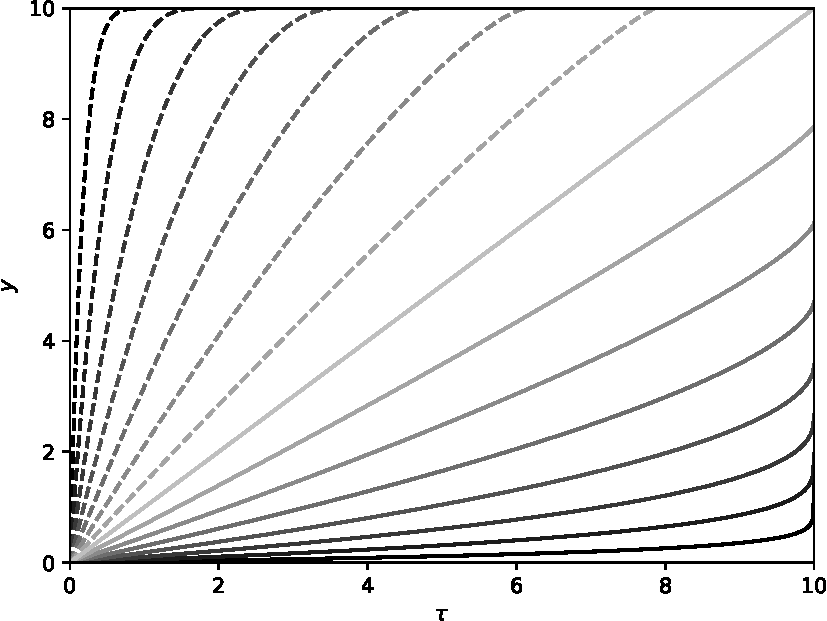
\includegraphics[width=0.75\textwidth]{gh.pdf}
\caption{This figure depicts the curves of $g_{10}^{\alpha}(\tau)$ and $h_{10}^{\alpha}(\tau)$ for $\alpha\in\mathsf{A}$. The curves associated with $g$ are plotted using 
solid lines, while the curves plotted wit h dashed lines are associated with $h$. The lighter the shade with which a curve is depicted, the larger the $\alpha$-value is that is associated with it.
}
\label{fig:gandh}
\end{figure}

\section{Existing Geometric Interpretation}
Podlubny suggested to build a ``fence'' in $(\tau,g_t^{\alpha},f)$-space. The base of the aforementioned fence is geiven by the curve $(\tau,g_t^{\alpha}(\tau),0)$, while its height is determined by $(\tau,g_t^{\alpha}(\tau),f(\tau))$. The 
``shadow'' of this fence, i.e. the area under the curve which is obtained by 
projecting this fence onto the $gf$- plane corresonds to the value which is obtained when Eq is evaluated. As an example, the visualization of  
\begin{equation}
xxx 
\end{equation}
using the fence-idea suggested by Podlubny is presented in Fig...


%geometric idea is depicted in Fig for $f(t)=\sqrt{t}$, $\alpha\in\{0.3,0.6,0.9\}$ and $\t\in\{3,6,9\}$. 


\begin{figure}[htb]
\centering
\includegraphics[width=1.0\textwidth]{vis_old.pdf}
\caption{This figure depicts the visualization of Eq using the geometric framework proposed by Podlubny.  The fence itstelf is depicted in green. The areas depicted in red (the shadow of the fence) correspond to the value obtained if Eq. is evaluated.  The surface which is obtained 
by extending the curve $f(\tau)$ and $g_t^{\alpha}(\tau)$ along the $g$ and $f$ direction 
is depicted in cyan and blue respectively. The curve that determines the height of the fence 
}
\label{fig:gandh}
\end{figure}


\section{Converting into a Cavalieri integral}

\begin{theorem}
Let $\widetilde{g}_t^{\alpha}=\frac{\left \{t^{\alpha} - (t-\tau)^{\alpha} \right \}}{\Gamma(\alpha+1)}$ and $a(y)_{t}^{\alpha} = f^{-1}(y) - \widetilde{g}_t^{\alpha}\circ f^{-1}(y) + \widetilde{g}_t^{\alpha}(a')$. If $a(y)_t^{\alpha}$ and $a(0)$ exists then  
there exists a $C\in \mathbb{R}$ such that the following integrals are geometrically equivalent:
\begin{equation}
\int_{a'}^{b'} f(x)\,dg_t^{\alpha}(x)~\textrm{and}~\int_{a_t^{\alpha}(y)}^{b_t^{\alpha}(y)} f(x)\,dx. 
\end{equation}
\end{theorem}





\noindent
Furthermore, Grobler showed that it is trivial to convert a Riemann-Stieltjes integral into a Cavalieri integral \cite{ackermann12,grobler19} (see Fig.~\ref{fig:caval2} and the Cavalieri section of this paper if more details are required). If we apply Grobler's conversion method to Eq.~\eqref{eq:rs} we obtain:
\begin{equation}
\label{eq:cav}
\int_{a_t^{\alpha}(y)}^{b_t^{\alpha}(y)} f(\tau)~d\tau, 
\end{equation}
with
\begin{equation}
\label{eq:cav_a}
a_t^{\alpha}(y) = f^{-1}(y) - \frac{t^{\alpha}-(t-f^{-1}(y))^{\alpha}}{\Gamma(\alpha+1)}.
\end{equation}
Eq.~\eqref{eq:cav_a} is obtained by substituting Eq.~\eqref{eq:g_rl} into Eq.~\eqref{eq:a_y}. Note, $b_t^{\alpha}(y) = a_t^{\alpha}(y) + \frac{t^{\alpha}}{\Gamma(\alpha+1)}$. 

\noindent
We can now assign a geometric interpretation to Eq.~\eqref{eq:cav}, since it is a Cavalieri integral (see Fig.~\ref{fig:caval2} and the Cavalieri section of this paper). The fractional integral in Eq.~\eqref{eq:RL_frac_int} can, therefore, be interpreted as the area obtained 
by summing together the area of an infinite number of infinitesimally small non-rectangular integration strips whose shape is determined by $\alpha$ and $t$. If $\alpha$ is equal to one, however, then the integral reduces to a normal Riemann integral as the integration strips become rectangular for this particular choice of $\alpha$ (its shape becomes independent of $t$).\\

\noindent
Interestingly, Eq.~\eqref{eq:main_cav} implies that we can use $h_t^{\alpha}(\tau)$ to convert Eq.~\eqref{eq:cav} into the following Riemann integral:
\begin{equation}
\label{eq:option2}
\int_0^{\frac{t^{\alpha}}{\Gamma(\alpha+1)}} f\circ h_{\alpha}^t (\tau) d\tau.  
\end{equation}
We can, therefore, evaluate Eq.~\eqref{eq:cav} in one of two ways: we can either evaluate Eq.~\eqref{eq:rs} or we can evaluate Eq.~\eqref{eq:option2}.


 
%%%%%%%%%%%%%%%%%%%%%%%%%%%%%%%%%%%%%%%%%%%%%%%%%
\section*{Acknowledgements}

 The author thanks his institution for the support, under Grant No ...

%%%%%%%%%% References %%%%%%%%%%%%%%%%%%%%%%%%%%%%%%%%
%%%% arranged in ALPHABETIC ORDER of Authors' Families
%%%% for articles, insert also DOI numbers if available

 \begin{thebibliography}{99}
 \normalsize

%%%% example for a book %%%%%%%%%%%%%

\bibitem{GasRah}
 G. Gasper, M. Rahman,
 \emph{Basic Hypergeometric Series}.
 Cambridge University Press, Cambridge (1990).

%%%% example for article in FCAA journal %%%%%%%%%%%%%%%%%

\bibitem{Kir}
 V. Kiryakova,
 A brief story about the operators of generalized
fractional calculus.
 \emph{Fract. Calc. Appl. Anal.} \textbf{11}, No 2 (2008), 201--218; DOI: ..........

%%%% example for journal's article %%%%%%%%%%%%%%%%%

\bibitem{Moak}
 D.S. Moak,
 The $q$-analogue of the Laguerre polynomials.
\emph{J. Math. Anal. Appl.} \textbf{81}, No 1 (1981), 20--47. % ; doi: ........

%%%% example for a paper in Proceedings %%%%%%%%%%%%%

\bibitem{Rosbl}
 M. Rosenblum,
 Generalized Hermite polynomials and the Bose-like oscillator
 calculus.
 In: \emph{Operator Theory: Advances and Applications},
 Birkh\"auser, Basel (1994), 369--396.
%%%%%%%%%%%%%%%%%%%%%%%%%%%%%%%%%%%%%%%%%%%%%%%%%%%%

\end{thebibliography} %%%%%%%%%%%%%%%%%%%%%%%%%%%%%%%%

%%%%%%%%%% put authors' addresses here, in \it %%%%%%%%

 \bigskip \smallskip

 \it

 \noindent
   %(First) Author's full postal address
$^1$ Institute of Mathematics and Informatics \\
Bulgarian Academy of Sciences \\
"Acad. G. Bontchev" Str., Block 8 \\
Sofia -- 1113, BULGARIA  \\[4pt]
  e-mail: virginia@diogenes.bg
\hfill Received: November 1, 2014 \\[12pt]
  % Second Author's address
$^2$ Dept. of Physics, University of Bologna\\
Via Irnerio 46, I -- 40126 Bologna, ITALY \\[4pt]
  e-mail: .....

\end{document} %%%%%%%%%%%%%%%%%%%%%%%%%%%%%%%%%%%%%
